% !TeX program = xelatex
\documentclass{article}

% ------- Packages and Settings --------
 
% GENERAL 

%
% Load KNMI poster package
%
% 	Options:
%
%	portrait* | landscape		set poster orientation
%	cmyk* | rgb		 	set pdf colour mode
% 	english* | dutch			set KNMI logo language
% 	epslogo* | pdflogo		set KNMI logo format
% 	disablefonts			disable all custom fonts (and the need for XeLaTeX)
% 	path			 		specify path to ?KNMIposter? (default = current directory)
% 	fixfooter			 	fix footer spacing (required for some Tex/Postscript versions)
% 	debug			 	enable geometry showframe
%
% * = default
%
\usepackage[landscape]{KNMIposter}


% USER PACKAGES
% language
\usepackage[english]{babel}

% Define path for figures -- for safety, keep the last /
\graphicspath{{example_figures/}}

% Assist LaTeX in hyphenation
\hyphenation{Rey-nold}
\hyphenation{Ra-ma-swa-my}


% USER PACKAGES
% language
\usepackage[english]{babel}

% Define path for figures -- for safety, keep the last /
\graphicspath{{EGU_figures/}}

% Assist LaTeX in hyphenation
\hyphenation{Rey-nold}
\hyphenation{Ra-ma-swa-my}

\usepackage{tcolorbox}



% ------- POSTER HEADER --------

% Poster title
\title{Automatic fog detection for public safety by using camera images}

% Author
\author{Giuliano Andrea Pagani\affil{1}, Martin Roth\affil{1}, and Wiel Wauben\affil{1}. Contact: \email{pagani@knmi.nl}}

% Affiliations
\affiliations{\affil{1}R\&D Department of Observations and Data-Technology, Royal Netherlands Meteorological Institute. PO Box 201, 3730 AE De Bilt, The Netherlands.%
}

% You can either add the contact information in the author line (poster top, large),
% or in the affiliations (poster bottom, footnote size).

% Some additional space for acknowledgements, url's, ... 
% \acknowledge{I would like to thank all of you!}


% ------- Document start --------
\begin{document}

\maketitle

\begin{abstract}
Visibility is traditionally measured manually by meteorological observers using landmarks at known distances in
the vicinity of the observation site. 
%Nowadays, distributed cameras facilitate inspection of more locations from one
%remote monitoring center. The main idea is, however, still deriving the visibility or presence of fog by an operator
%judging the scenery and the presence of landmarks. 
Visibility sensors are also used, but they are rather costly and
require regular maintenance. Moreover, observers, and in particular sensors, give only visibility information that is
representative for a limited area. 
Cameras are more and more deployed for surveillance and security reasons in cities and for monitoring traffic along
main transportation routes. In addition to this primary use of cameras, we consider cameras as potential sensors to
automatically identify low visibility conditions. 
The approach that we follow is to use machine learning techniques
to determine the presence of fog or to make an estimation of the visibility. 
%For that purpose a set of features
%are extracted from the camera images such as the number of edges, brightness, transmission of the image dark
%channel, fractal dimension. In addition to these image features, we also consider meteorological variables such
%as wind speed, temperature, relative humidity, and dew point as additional features to feed the machine learning
%model. %Furthermore, it is shown how to generate a pdf file which can easily be handled by the studio for printing.
\end{abstract}

\bcols %% Start columns

\section*{Motivation}
Fog and reduced visibility have considerable impact on the performance of road, maritime, and aeronautical transportation
networks. The impact ranges from minor delays to more serious congestions or unavailability of the
infrastructure and can even lead to damage or loss of lives~\cite{gultepe2007fog}.

%\vspace{-0.5cm}
\begin{minipage}[b]{\columnwidth}
	\begin{center}
	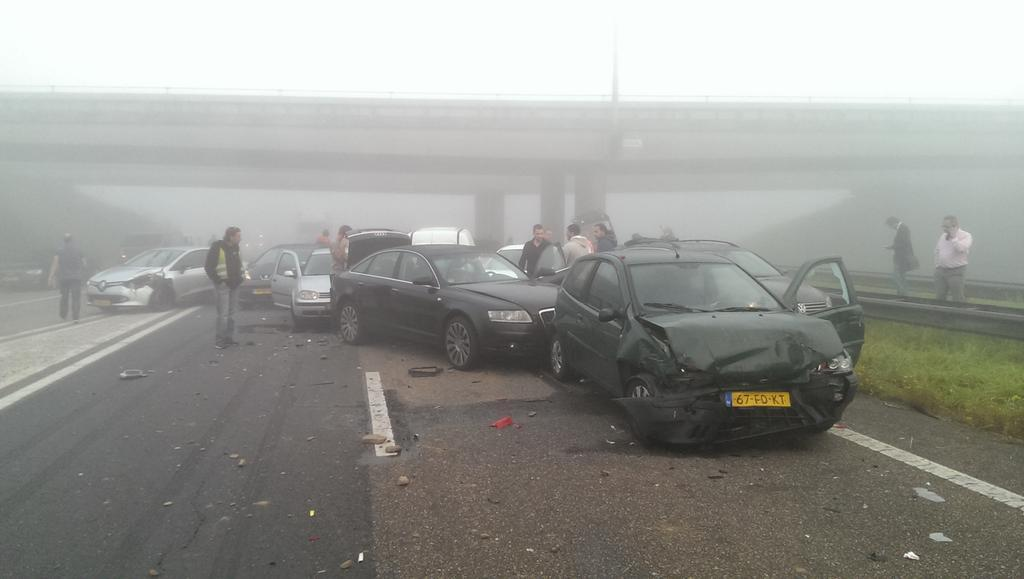
\includegraphics[width=0.9\columnwidth]{Accident}
	\captionof{figure}{Traffic accident caused by dense fog.}
	\label{figAccident}
	\end{center}
\end{minipage}
\vspace{-2cm}

\subsection*{Key facts about fog:}
\begin{itemize}
  \item May form and dissipate suddenly.
  \item Often only a local phenomenon.
\end{itemize}

\subsection*{Limitations of current technology:}
\begin{itemize}
\item Weather stations observe a limited area.
\item Satellites are not constantly observing areas of interest.
\item Forecast of fog conditions is complex.
\end{itemize}

\subsection*{Idea:}
Use cameras deployed for surveillance and security reasons in cities and for monitoring traffic along
main transportation routes as potential sensors to
automatically identify low visibility conditions.


\begin{minipage}[b]{\columnwidth}
\centering
\begin{minipage}[b]{0.4\columnwidth}
	\begin{center}
	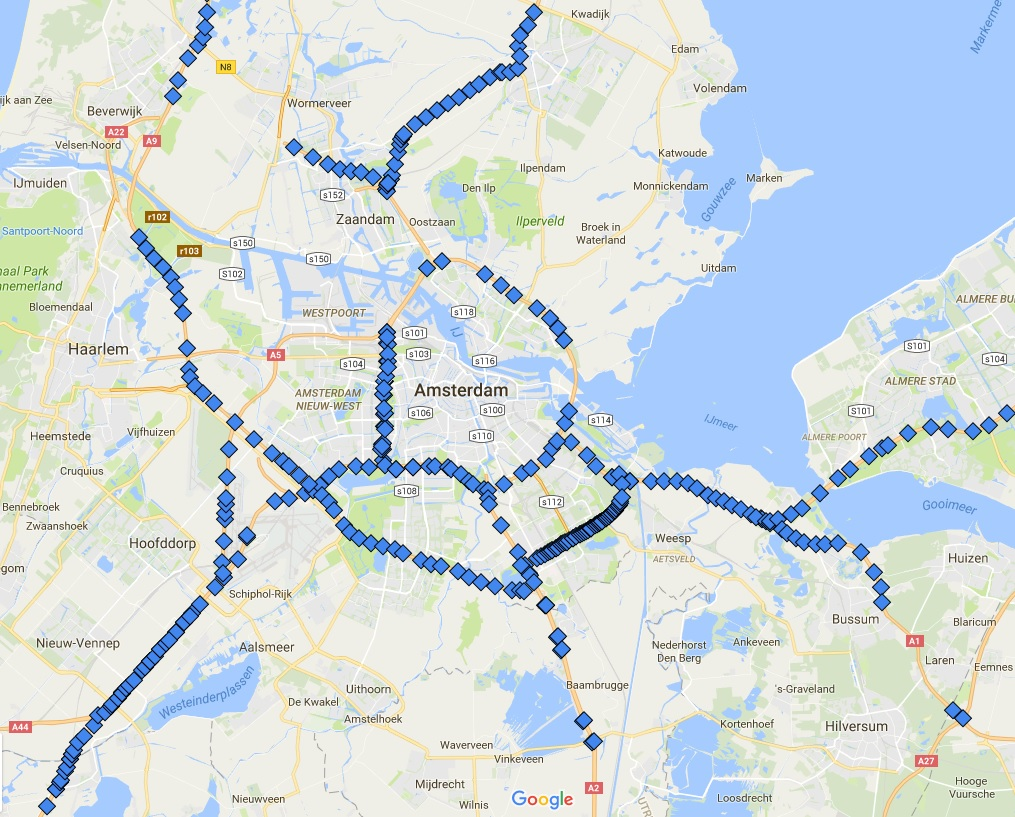
\includegraphics[width=\columnwidth]{CameraPlacement}
	\captionof{figure}{Cameras monitoring highways in Amsterdam region.}
	\label{figCameras}
	\end{center}
	\end{minipage}
	\hspace*{0.1cm}
\begin{minipage}[b]{0.4\columnwidth}
	\begin{center}
	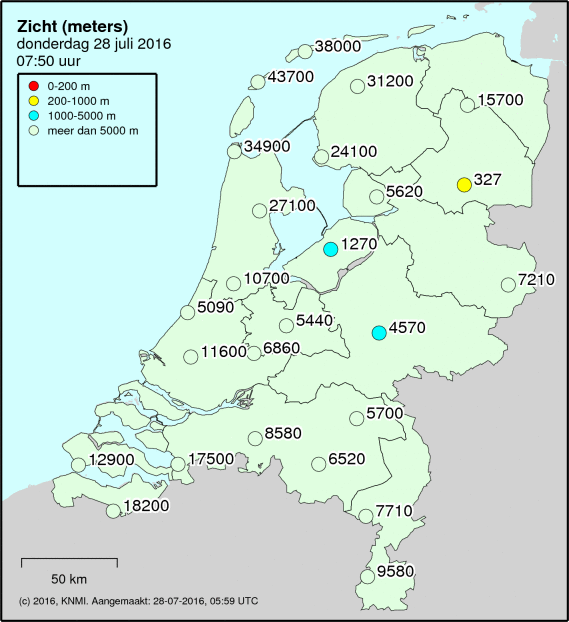
\includegraphics[width=\columnwidth]{SensorPlacement}
	\captionof{figure}{KNMI weather stations measuring visibility.}
	\label{figSensors}
	\end{center}
\end{minipage}
\end{minipage}

\section*{Approach}
% \subsection*{From Images to Machine Learning}
General properties of the images (\textbf{features}) are computed. 
Properties that are expected to vary with visibility conditions are:

\begin{tcolorbox}[colback=red!5!white,colframe=red!75!black,title=Image Features]
\begin{itemize}
\item{Mean Edges: determining the boundaries of objects within images. 
More edges (e.g., foreground and background elements or horizon) indicate better
visibility.
}
\item{Mean Brightness: perception of the luminance of sources of radiating/reflecting light.}
\item{Mean Saturation: is a measure of the purity of the color. 
The purest (most saturated) colors are obtained in the absence of atmospheric turbidity.
}
\item{Mean HUE: perception of a source of being similar to one of the perceived colors: red, yellow, green, and blue, or to a combination of two of them.}
\item{Fractal Dimension: self similarity in filling space.}
\item{Transmission smoothness: transmission of the dark channel of the image.}
\item{Transmission changepoint: horizontal point where the transmission of the dark channel is subject to change.}
\end{itemize}
%\item{Weather based:}
%\begin{itemize}
%\item{Wind speed}
%\item{Dew point}
%\item{Humidity}
%\item{Precipitation amount}
%\end{itemize}
%\end{itemize}
\end{tcolorbox}


%Pictures are translated to a set of quantities capturing their properties (\textbf{features}).\newline
The measurements obtained by a nearby forward scatter sensor is considered the
reference for the visibility conditions \emph{in the measurement field}
(\textbf{supervised} problem).\newline
A classifier is trained with the features extracted from the images and the 
visibility (class) provided by the sensor.
\vspace*{0.8cm}

\textit{Restrictions}: 
i) static cameras,
ii) daylight conditions,
iii) period: 3/2015 - present, 
iv) image sampling time: 10 minutes.




\begin{minipage}[b]{\columnwidth}
	\begin{center}
	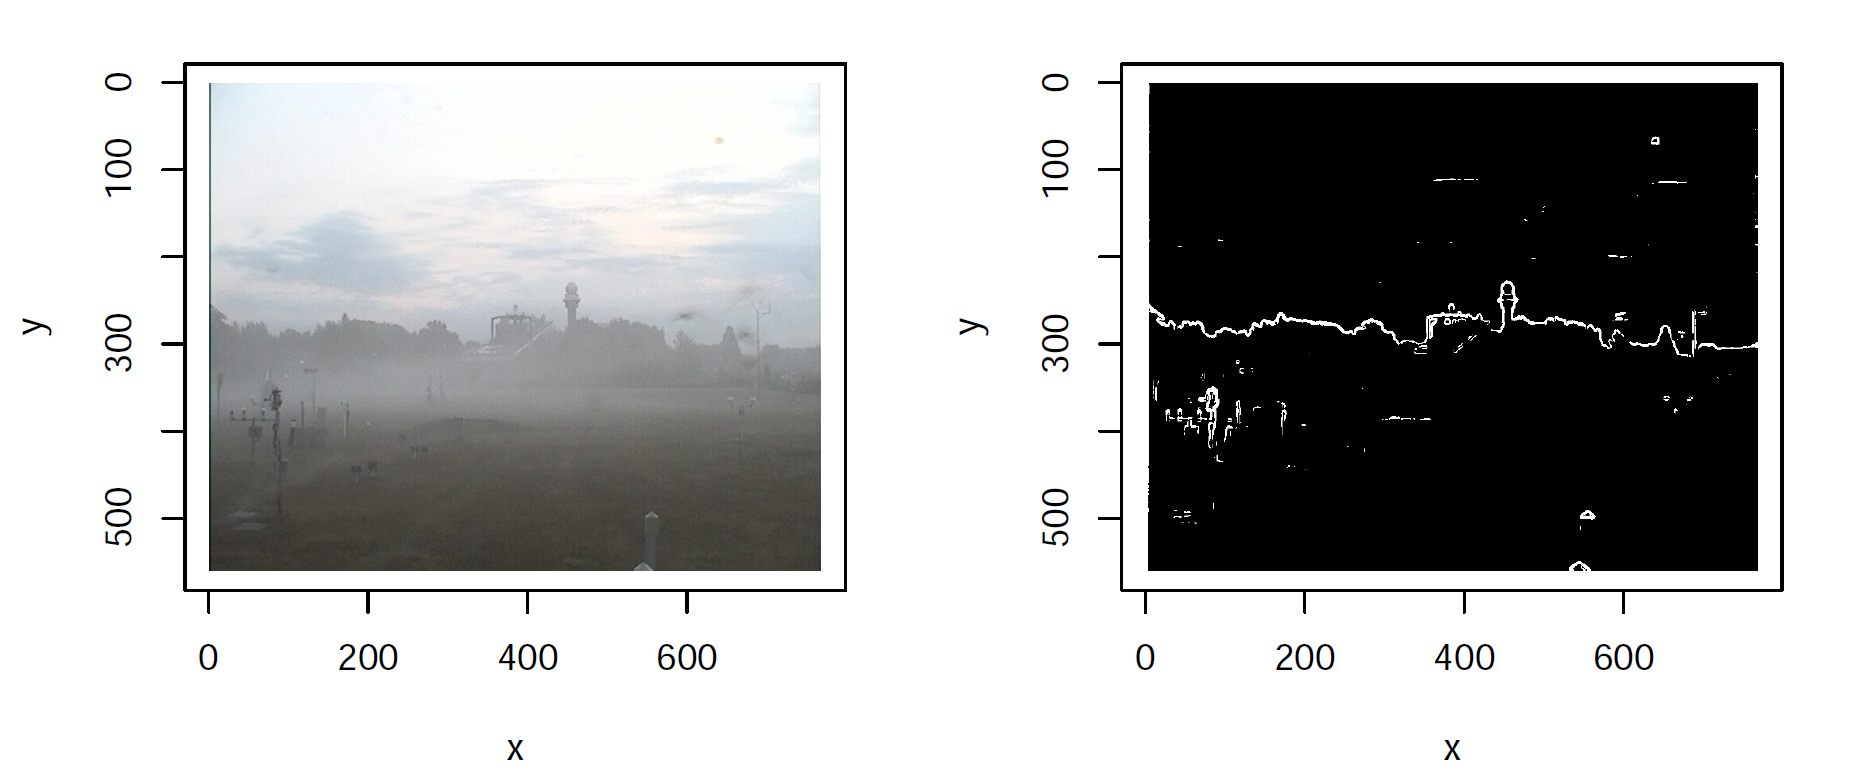
\includegraphics[width=0.95\columnwidth]{edges}
	\captionof{figure}{Edges in images.}
	\label{figEdges}
	\end{center}
\end{minipage}

\begin{minipage}[b]{\columnwidth}
	\begin{center}
	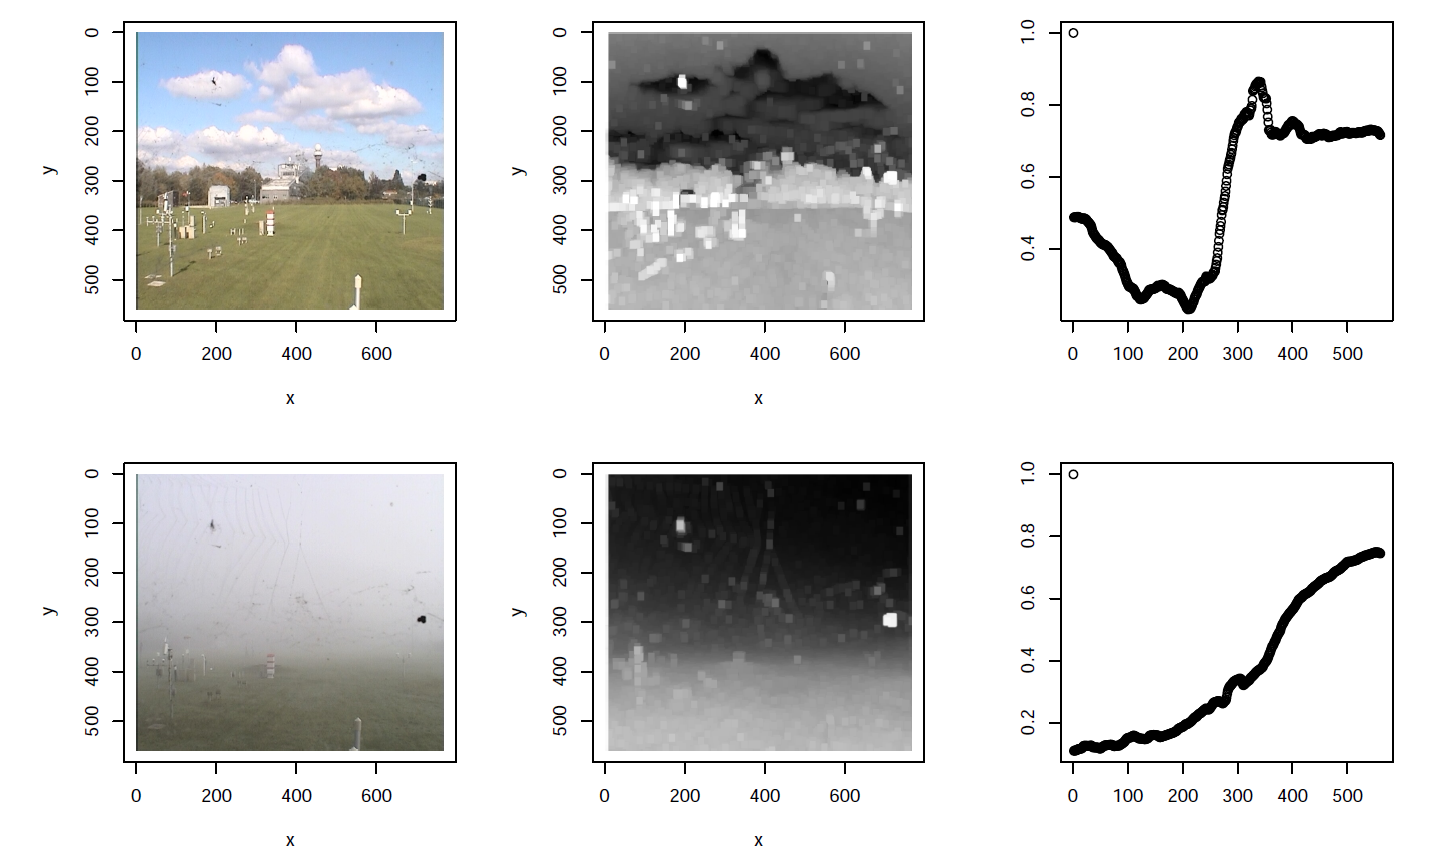
\includegraphics[width=0.95\columnwidth]{transmission}
	\captionof{figure}{Average horizontal dark channel transmission: clear (top) and foggy (bottom) day.}
	\label{figTransmission}
	\end{center}
\end{minipage}
\vspace*{-5cm}


\section*{Results}
The initial goal to identify fog conditions from images has been achieved using \textbf{Decision Tree} technique. This is to be considered a first step to improve upon. We aim to identify fog in more advanced and complex dynamic scenarios.

\begin{minipage}[b]{\columnwidth}
	\begin{center}
	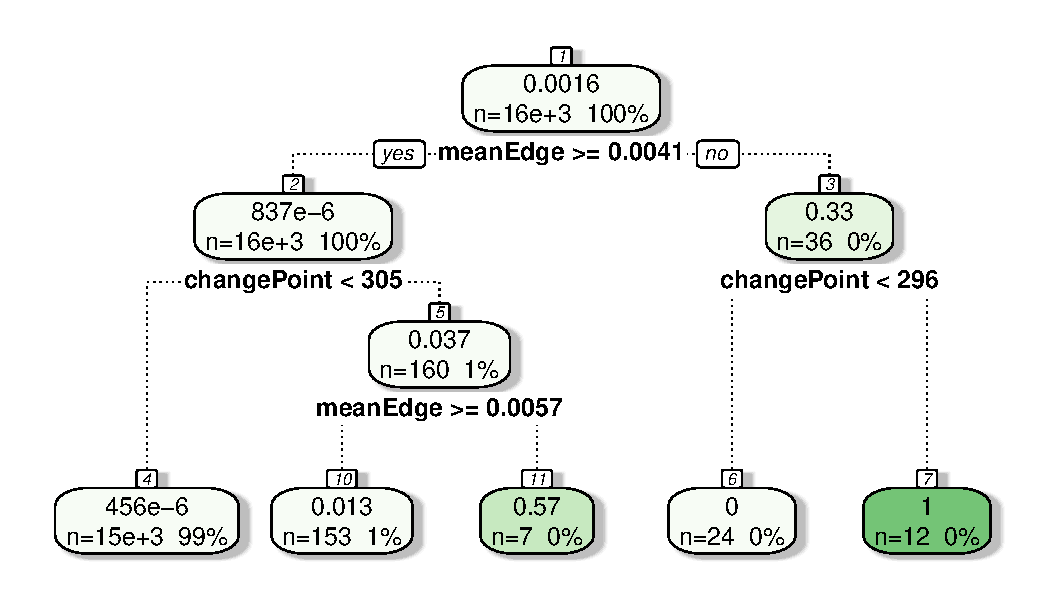
\includegraphics[width=0.9\columnwidth]{ClassificationTree-1}
	\captionof{figure}{Decision Tree results for De Bilt training set.}
	\label{figTree}
	\end{center}
\end{minipage}
For location De Bilt the result are promising in the training (March-December 2015) and the test set (January-June 2016) in terms of \textbf{Probability of Detection} and \textbf{False Alarm Ratio}.
\begin{tcolorbox}[colback=red!5!white,colframe=red!75!black,title=Overall Project Results]
\begin{itemize}
\item{Partnership with governmental institution for road management.}
\item{Access to traffic monitoring cameras on Dutch highways.}
\item{Access to observation cameras in Dutch airports.}
\item{Processing of images in distributed infrastructure on AWS cloud.}
\item{Creation of a R image features processing library \url{https://github.com/MartinRoth/visDec}}
\end{itemize}
\end{tcolorbox}
\begin{minipage}[b]{\columnwidth}
	\begin{center}
	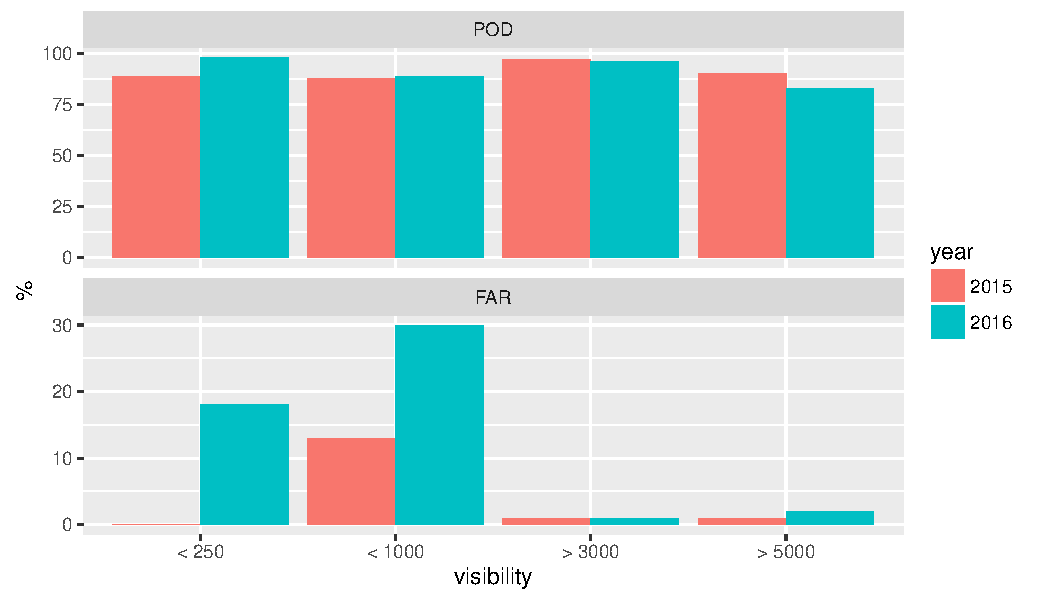
\includegraphics[width=0.9\columnwidth]{PODandFAR3-1}
	\captionof{figure}{POD-FAR for De Bilt training (2015) and test (2016)}
	\label{figTree}
	\end{center}
\end{minipage}





%\columnbreak % force jump to next column


\section*{Follow up - Open Questions}
There are plenty of aspects we are working or planning to work on:
\begin{enumerate}
\item Analyze images from more locations. \newline
Other KNMI locations with cameras have been used (weather station Twente, Cabauw). More locations are now available at airports and highways.
\item Addition of meteorological features to image-only features.\newline
Some initial investigations have been performed in adding meteorological conditions and having a more broad feature space.
\item Addition of spatial and temporal relationship in the fog estimation.
\item How to deal with dawn conditions? Can an image-based approach be used also at night?
\item How to generalize static cameras approach to a dynamic scene? And to a totally different scene?\newline
Master student project in collaboration with University of Amsterdam applying domain adaptation techniques~\cite{ganin2016domain} to identify a set of features from different scenes that can be used to any (new) scene.
\end{enumerate}


% Figure
% \vspace{20pt plus 10pt minus 5pt}
% \begin{minipage}[b]{\columnwidth}\begin{center}
% 	\begin{center}
% 	\includegraphics[width=\columnwidth]{fig2}
% 	\captionof{figure}{Part of an AVIRIS flight line acquired over the Pacific Ocean. Left half: a water cloud (Sc), right half: an ice cloud (Ci).}
% 	\label{fig2}
% 	\end{center}
% \end{center}\end{minipage}


%\pushdown


\bibliographystyle{IEEEtran}


\bibliography{biblio}


\ecols %% End columns 

\end{document}
